\documentclass[12pt, twoside]{article}
\documentclass[12pt, twoside]{article}
\usepackage[letterpaper, margin=1in, headsep=0.2in]{geometry}
\setlength{\headheight}{0.6in}
%\usepackage[english]{babel}
\usepackage[utf8]{inputenc}
\usepackage{microtype}
\usepackage{amsmath}
\usepackage{amssymb}
%\usepackage{amsfonts}
\usepackage{siunitx} %units in math. eg 20\milli\meter
\usepackage{yhmath} % for arcs, overparenth command
\usepackage{tikz} %graphics
\usetikzlibrary{quotes, angles}
\usepackage{graphicx} %consider setting \graphicspath{{images/}}
\usepackage{parskip} %no paragraph indent
\usepackage{enumitem}
\usepackage{multicol}
\usepackage{venndiagram}

\usepackage{fancyhdr}
\pagestyle{fancy}
\fancyhf{}
\renewcommand{\headrulewidth}{0pt} % disable the underline of the header
\raggedbottom
\hfuzz=2mm %suppresses overfull box warnings

\usepackage{hyperref}
\usepackage{float}

\fancyhead[LE]{\thepage}
\fancyhead[RO]{\thepage \\ First and last name: \hspace{2.5cm} \,\\ Section: \hspace{2.5cm} \,}
\fancyhead[LO]{BECA / Dr. Huson / Regents Prep: Graphs\\* 12 November 2024}

\begin{document}

\subsubsection*{3.1 Do Now: Graphing quadratic systems}
\begin{enumerate}
  \item The quadratic of a system of equations is graphed. Add a graph of the linear equation. Mark the intersections as ordered pairs.

  \begin{multicols}{2}
    $y = x^2 - x - 1$ \\
    \columnbreak
    $y = x + 2$
    \end{multicols}
    What values of $x$ satisfy the system of equations? \vspace{2cm}

  \begin{center}
  \begin{tikzpicture}[scale=.635]
    \draw [help lines] (-10,-10) grid (10,10);
    \draw [thick, ->] (-10.2,0) -- (10.4,0) node [below right] {$x$};
    \draw [thick, ->] (0,-10.2)--(0,10.4) node [left] {$y$};
    \draw[thick, domain=-2.7:3.7] plot (\x, {(\x)^2 - \x - 1});
  \end{tikzpicture}
  \end{center}

\newpage
\item Circle the equations that are an identities.
    \begin{multicols}{2}
      \begin{enumerate}
        \item \(x^2 + y^2 = (x + y)^2\)
        \item \(x^2 - y^2 = x^2 - 2xy + y^2\)
        \item \(x^3 - y^3 = (x + y)(x^2 - xy + y^2)\)
        \item \(x^3 + y^3 = (x + y)(x^2 - xy - y^2)\)
      \end{enumerate}
    \end{multicols}

\item Write a recursive definition of the sequence $a_1 = -3$, $a_2 = -9$, $a_3 = -12$, $a_4 = -15, \ldots$ \vspace{2cm}
    
\item Write down the solutions to the equation $(2x-7)(x - 5)(x - 1) = 0$ \vspace{2cm}

\item Graphed is $f(x) = x^3-6x^2+3x+8$. Write the function in factored form. 
    \begin{flushright}
    \begin{tikzpicture}[xscale=1, yscale=0.25]
        \draw [thick, ->] (-3.2,0) -- (5,0) node [above] {$x$};
        \draw [thick, ->] (0,-9.2)--(0,10) node [right] {$y$};
        \foreach \x in {-3,...,4} \draw (\x cm,12pt) -- (\x cm,-12pt) node[below] {$\x$};
        \foreach \y in {-8,-4,4,8} \draw (3pt,\y cm) -- (-3pt,\y cm) node[left] {$\y$};
        \draw [thick, <->,smooth,samples=20,domain=-2.3:4.2] plot(\x,{(\x+2)*(\x-1)*(\x-4)});
    \end{tikzpicture}
    \end{flushright}

\item Solve algebraically for $n$: $\displaystyle \frac{2}{n^2} + \frac{3}{n} = \frac{4}{n^2}$ %June 2022 Regents
\vspace{4cm}


\end{enumerate}
\end{document}